% Start of Chapter 2 - Mathematical development

Through the numerous literature it is possible to find several approaches to obtain a model for the Inverted Pendulum elements. For this work the focus is mostly on the dynamic behavior of the robot, as it is the one that influences the most the response of the system. To completely model the dynamic behavior of the robot, we need to consider the equations that govern the movement as a rigid body.

\section{First approach: Sum of forces}

The first approach considered here is described in \cite{SUL03}. The methodology uses traditional dynamic physics to obtain the equations of motion. The final equation is then linearized and transformed into complex frequency domain.

\subsection{Dynamic behavior}

The equations of motion are obtained from the sum of forces in the cart for the horizontal direction (see figure \ref{fig:carforces}).

\begin{figure}[h]
	\centering
	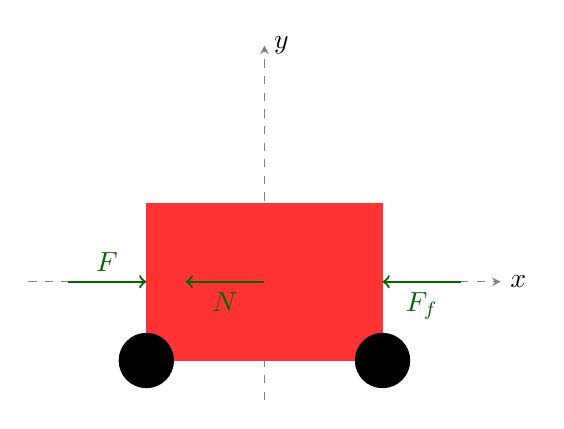
\begin{tikzpicture}
		[force/.style={->,thick,green!40!black}]
		% draw the two coordinate axis
		\draw [dashed,>=stealth,->, draw=gray] (-3,0) -- (3,0) node[anchor=west]{$x$};
		\draw [dashed,>=stealth,->, draw=gray] (0,-1.5) -- (0,3) node[anchor=west]{$y$};

		% draw the red mass with two wheels
		\fill[red!80!white] (-1.5,-1) rectangle (1.5,1);
		\fill (-1.5,-1) circle [radius=10pt];
		\fill (1.5,-1) circle [radius=10pt];

		%draw the forces
		\draw [force] (-2.5,0) -- node[green!40!black, auto]{$F$} (-1.5,0);
		\draw [force] (2.5,0) -- node[green!40!black, auto]{$F_f$} (1.5,0);
		\draw [force] (0,0) -- node[green!40!black, auto]{$N$} (-1,0);
	\end{tikzpicture}
	\caption{Cart forces}\label{fig:carforces}
\end{figure}

\begin{equation} \label{sfch}
	F-b\cdot \dot{x}-N=M\cdot \ddot{x}
\end{equation}

Now considering the pendulum itself, the force applied in the horizontal direction due to the momentum of the pendulum is determined as:

\begin{figure}[h]
	\centering
	\begin{tikzpicture}
		[force/.style={->,thick,green!40!black}]
		% draw the two coordinate axis
		\draw [dashed,>=stealth,->, draw=gray] (-3,0) -- (3,0) node[anchor=west]{$x$};
		\draw [dashed,>=stealth,->, draw=gray] (0,-1.5) -- (0,3) node[anchor=west]{$y$};

		% draw the pendulum
		\node [circle,draw,blue,inner sep=0pt,minimum size=20pt] (pen) at (70:3) {};
		\draw[blue] (0,0) -- (pen);

		%draw the forces
		\draw [force] (-2.5,0) -- node[green!40!black, auto]{$F$} (-1.5,0);
	\end{tikzpicture}
	\caption{Pendulum forces}\label{fig:penforces}
\end{figure}

\begin{equation} \label{dhfp}
	\tau=r\cdot F=I\cdot \ddot{\theta}
\end{equation}

Given the fact that the moment of inertia of a pendulum of mass $m$ is defined as $I=m\cdot L^2$, the previous equation can be rewritten as:

\begin{equation} \label{dhfp2}
	F=\frac{I\cdot \ddot{\theta}}{r}=\frac{m\cdot l^2\cdot \ddot{\theta}}{l}=m\cdot l\cdot \ddot{\theta}
\end{equation}

Obtaining the component of the force defined in \ref{dhfp2} in the horizontal direction:

\begin{equation} \label{sfph}
	F=m\cdot l\cdot \ddot{\theta}\cdot \cos{\theta}
\end{equation}

Now, the component of the centripetal force acting on the pendulum is similar to the one in \ref{dhfp2}, but the horizontal component of this force is:

\begin{equation} \label{cfph}
	F=m\cdot l\cdot \dot{\theta}^2\cdot \sin{\theta}
\end{equation}

Summing the defined forces present in the horizontal direction of the pendulum in \ref{sfph} and \ref{cfph}, we obtain the following expression:

\begin{equation} \label{nfp}
	N=m\cdot \ddot{x}+m\cdot l\cdot \ddot{\theta}\cdot \cos{\theta}-m\cdot l\cdot \dot{\theta}^2\cdot \sin{\theta}
\end{equation}

Now we can substitute \ref{nfp} into \ref{sfch}, we obtain the first equation of motion:

\begin{equation} \label{fem}
	F=(M+m)\ddot{x}+b\cdot \dot{x}+m\cdot l\cdot \ddot{\theta}\cdot \cos{\theta}-m\cdot l\cdot \dot{\theta}^2\cdot \sin{\theta}
\end{equation}

To get the second equation of motion, we sum the forces perpendicular to the pendulum. The vertical components of this forces are considered here to get:

\begin{equation} \label{sfppv}
	P\cdot \sin{\theta}+N\cdot \cos{\theta}-m\cdot g\cdot \sin{\theta}=m\cdot l\cdot \ddot{\theta}+m\cdot \ddot{x}\cdot \cos{\theta}
\end{equation}

To get rid of the $P$ and $N$ terms, sum the moments around the center of gravity of the pendulum:

\begin{equation} \label{smcg}
	-P\cdot l\cdot \sin{\theta}-N\cdot l\cdot \cos{\theta}=I\cdot \ddot{\theta}
\end{equation}

Summing up the equations \ref{sfppv} and \ref{smcg}, we obtain the second equation of movement:

\begin{equation} \label{sem}
	(I+m\cdot l^2)\ddot{\theta}+m\cdot g\cdot l\cdot \sin{\theta}=-m\cdot l\cdot \ddot{x}\cdot \cos{\theta}
\end{equation}

The obtained equations are non-linear, so they are linearized around the operating point, defined as the top vertical position or $\pi rad$ from the stable equilibrium position. We need also to define a small angle deviation from the top vertical position, so that $\theta=\pi+\phi$.

Under this circunstances, we can deduce that $\cos{\theta}\approx -1$, $\sin{\theta}\approx -\phi$, and $\dot{\theta}^2\approx 0$. Applying this relations into our movement equations, we obtain:

\begin{equation} \label{feml}
	F=(M+m)\ddot{x}+b\cdot \dot{x}-m\cdot l\cdot \ddot{\phi}
\end{equation}

\begin{equation} \label{seml}
	(I+m\cdot l^2)\ddot{\phi}-m\cdot g\cdot l\cdot \phi=m\cdot l\cdot \ddot{x}
\end{equation}

To obtain the transfer function of the linearized system of equations analytically, we perform the Laplace transform of the system equations:

\begin{equation} \label{fems}
	F(s)=(M+m)s^2\cdot X(s)+b\cdot s\cdot X(s)-m\cdot l\cdot s^2\cdot \Phi(s)
\end{equation}

\begin{equation} \label{sems}
	(I+m\cdot l^2)s^2\cdot \Phi(s)-m\cdot g\cdot l\cdot \Phi(s)=m\cdot l\cdot s^2\cdot X(s)
\end{equation}

To unify the equations, we solve \ref{fems} for $X(s)$ and then replace it into \ref{sems}, obtaining:

\begin{equation} \label{ecms}
	\frac{\Phi(s)}{F(s)}=\frac{m\cdot l\cdot s}{q\cdot s^3+b(l+m\cdot l^2)s^2-m\cdot g\cdot l(M+m)s-b\cdot m\cdot g\cdot l}
\end{equation}

Where:

\begin{equation} \label{dq}
	q=(M+m)(l+m\cdot l^2)-(m\cdot l)^2
\end{equation}

Assuming a coefficient of friction as zero, we can represent the equation as:

\begin{equation} \label{efms}
	\frac{\Phi(s)}{F(s)}=\frac{K_p}{\frac{s^2}{A_p^2}-1}
\end{equation}

With:

\begin{equation} \label{dka}
	K_p=\frac{1}{(M+m)g} ; A_p=\pm \sqrt{\frac{(M+m)m\cdot g\cdot l}{(M+m)(l+m\cdot l^2)-(m\cdot l)^2}}
\end{equation}

\subsection{Actuator system}

The actuation mechanism consist on a DC motor that drives a belt sytem around two wheels. The overall transfer function of the actuation mechanism will depend upon the motor and the belt system.

The torque to be delivered by the motor is:

\begin{equation} \label{t}
	T_L=(M+m)r^2\dot{\omega}
\end{equation}

The relation between Torque and Force can be expressed as:

\begin{equation} \label{dtf}
	T_L\propto r^2 ; F\propto r
\end{equation}

The motor dynamics can be represented with the well known tansfer function:

\begin{equation} \label{md}
	\omega(s)=K_m\frac{V(s)}{\tau s+1}
\end{equation}

Where $\tau$ is the time constant and depends on the load, and $K_m$ is the steady-state gain of the motor.

\begin{equation} \label{mtf}
	\frac{F(s)}{E(s)}=K_m\frac{(M+m)r\cdot s}{\tau s+1}
\end{equation}

\section{Second approach - Euler-Lagrange}

To represent the dynamics of the system as in \cite{JER12} and \cite{LUN02}, the initial definition is the natural form of the Lagrangian in classical mechanics:

\begin{equation} \label{nfl}
	\mathcal{L}=E_k-E_p
\end{equation}

Where $E_k=\frac{1}{2}mv^2$ and $E_p=mgh$. Equation \ref{nfl} can then be rewriten as:

\begin{equation} \label{nflr}
	\mathcal{L}=\frac{1}{2}mv^2-mgh
\end{equation}

The Euler-Lagrange equation states that:

\begin{equation} \label{ele}
	\frac{d}{dt}\left( \frac{\partial\mathcal{L}}{\partial\dot{\theta}} \right)=\frac{\partial\mathcal{L}}{\partial\theta}
\end{equation}

The pendulum is a stiff bar of lenght L which is supported at one end by a frictionless pin.

TODO: Insert image

From the figure we can state that:

\begin{equation} \label{coord}
	\begin{aligned}
		x&=L\sin{\theta} & \dot{x}&=L\cos{\theta}\dot{\theta}\\
		y&=L\cos{\theta} & \dot{y}&=-L\sin{\theta}\dot{\theta}
	\end{aligned}
\end{equation}

Velocity is a vector representing the change in the position in the coordinates $x$ and $y$. Hence:

\begin{equation} \label{vel}
	v^2=\dot{x}^2+\dot{y}^2
\end{equation}

With the coordinates found in \ref{coord}, we can substitute in \ref{vel} to obtain:

\begin{equation} \label{vels}
	\begin{split}
		v^2&=L^2\cos{\theta}^2\dot{\theta}^2+L^2\sin{\theta}^2\dot{\theta}^2\\
		v^2&=L^2\dot{\theta}^2
	\end{split}
\end{equation}

Substituting \ref{coord} and \ref{vels} into \ref{nflr}, we obtain:

\begin{equation} \label{les}
	\mathcal{L}=\frac{1}{2}mL^2\dot{\theta}^2-mgL\cos{\theta}
\end{equation}

To perform the Euler-Lagrange equation presented in \ref{ele}, we need to compute the partial derivatives. First we compute the left part:

\begin{equation} \label{dlrt}
	\frac{\partial\mathcal{L}}{\partial\theta}=mgL\sin{\theta}
\end{equation}

Now we compute the inner part of the right element:

\begin{equation} \label{dlrtd}
	\frac{\partial\mathcal{L}}{\partial\dot{\theta}}=mL^2\dot{\theta}
\end{equation}

And now we can compute the outer derivative of \ref{dlrtd}:

\begin{equation} \label{dlrtt}
	\frac{d}{dt}\left( \frac{\partial\mathcal{L}}{\partial\dot{\theta}} \right)=mL^2\ddot{\theta}
\end{equation}

Now that we have all the terms, we can write the equation:

\begin{equation} \label{eles}
	\begin{split}
		\frac{d}{dt}\left( \frac{\partial\mathcal{L}}{\partial\dot{\theta}} \right)&=\frac{\partial\mathcal{L}}{\partial\theta}\\
		mL^2\ddot{\theta}&=mgL\sin{\theta}\\
		\ddot{\theta}&=\frac{g}{l}\sin{\theta}
	\end{split}
\end{equation}

TODO: Insert development of second part of angular acceleration

The total accelerations present on the pendulum can then be stated as:

\begin{equation} \label{saa}
	\ddot{\theta}=\ddot{\theta}_g+\ddot{\theta}_x=\left(\frac{g}{l}\right)\sin{\theta}-\left(\frac{\dot{x}}{l}\right)\cos{\theta}
\end{equation}

The obtained equation is non-linear, so we apply an approximation based on the fact that the operation point implies an angle $\theta\approx0$. It means that $\sin{\theta}\approx\theta$ and $\cos{\theta}\approx1$. Applying this on \ref{saa}, we obtain:

\begin{equation} \label{lesa}
	l\ddot{\theta}-g\theta=-\ddot{x}
\end{equation}

To obtain the transfer function, we perform the Laplace transform on \ref{lesa}:

\begin{equation} \label{ltsa}
	ls^2\Theta(s)-g\Theta(s)=-s^2X(s)
\end{equation}

Now we solve for the variables $\Theta$ and $X$:

\begin{equation} \label{tfsa}
	ls^2\Theta(s)-g\Theta(s)=-s^2X(s)
\end{equation}

TODO: Complete
